\section[TCE- and cis-DCE-degradation for zero valent iron surface (1D)]{1D reactive transport: Competition of TCE- and cis-DCE-degradation for the zero valent iron surface}
\label{l_s_benchmark_1d_TCEonIon}

\subsection{Definition}
This example simulation demonstrates the use of \GeoSys for simulation of multi-species kinetic reactions. The reaction system was set up by D. {Sch\"afer} and published in \cite{Schaefer:2003}. Further, it was used for model verification of the newly implemented and developed kinetic reaction module in \GeoSys. The example considers flow in a one-dimensional column of 1 m length, resembling the thickness of a reactive iron barrier perpendicular to the flow direction. It involves 19 species and and 16 different geochemical reactions, both first-order degradation reactions of adsorbed substances and kinetic sorption reactions of the langmuir-type, considering competition for the available sorption sites.

The model set up consists of a 1d column with saturated ground water flow with a darcy velocity of 5.0$\times$ 10$^{-4}$ m d$^{-1}$ from left to right. Geochemical species are added to the inflowing water, and their sorption and degradation behavior is modeled. For a complete description of input parameters see the paper by {Sch\"afer} et al. (2003). Every degradation reaction follows a Langmuir-Hinshelwood-Hougen-Watson kinetics with a limited number of sites for the adsorption and desorption of chlorinated hydrocarbons on the reactive iron surface. Since all the reactive substances involved have to adsorb onto the reactive iron surface in order to be degraded, a competition for the surface sites occurs. This competition has been investigated in column studies and the observed concentration profiles were simulated with the numerical model TBC \cite{Schaefer:2003}.

Model results are compared an older version of \GeoSys, which was compared to the original TBC simulations.

\subsection{Solution}

Results of the simulation are shown in Fig.~\ref{profiles_TCEonIon}, where profiles of the dissolved species are shown. TCE and cis-DCE are added to the inflowing water. They compete for the sorption sites, and when sorbed degrade according to a first order degradation reaction. The retardation of the reactive species compared to the conservative tracer \texttt{mobile} is clearly visible. Also, just downstream of the concentration decrease of TCE or cis-DCE, the degradation products ethane and C4-containing molecules increase. These species are again mobile and are transported with the water, so an instationary behaviour is observed in Fig.~\ref{profiles_TCEonIon}.

\begin{figure}[htbp]
\centering
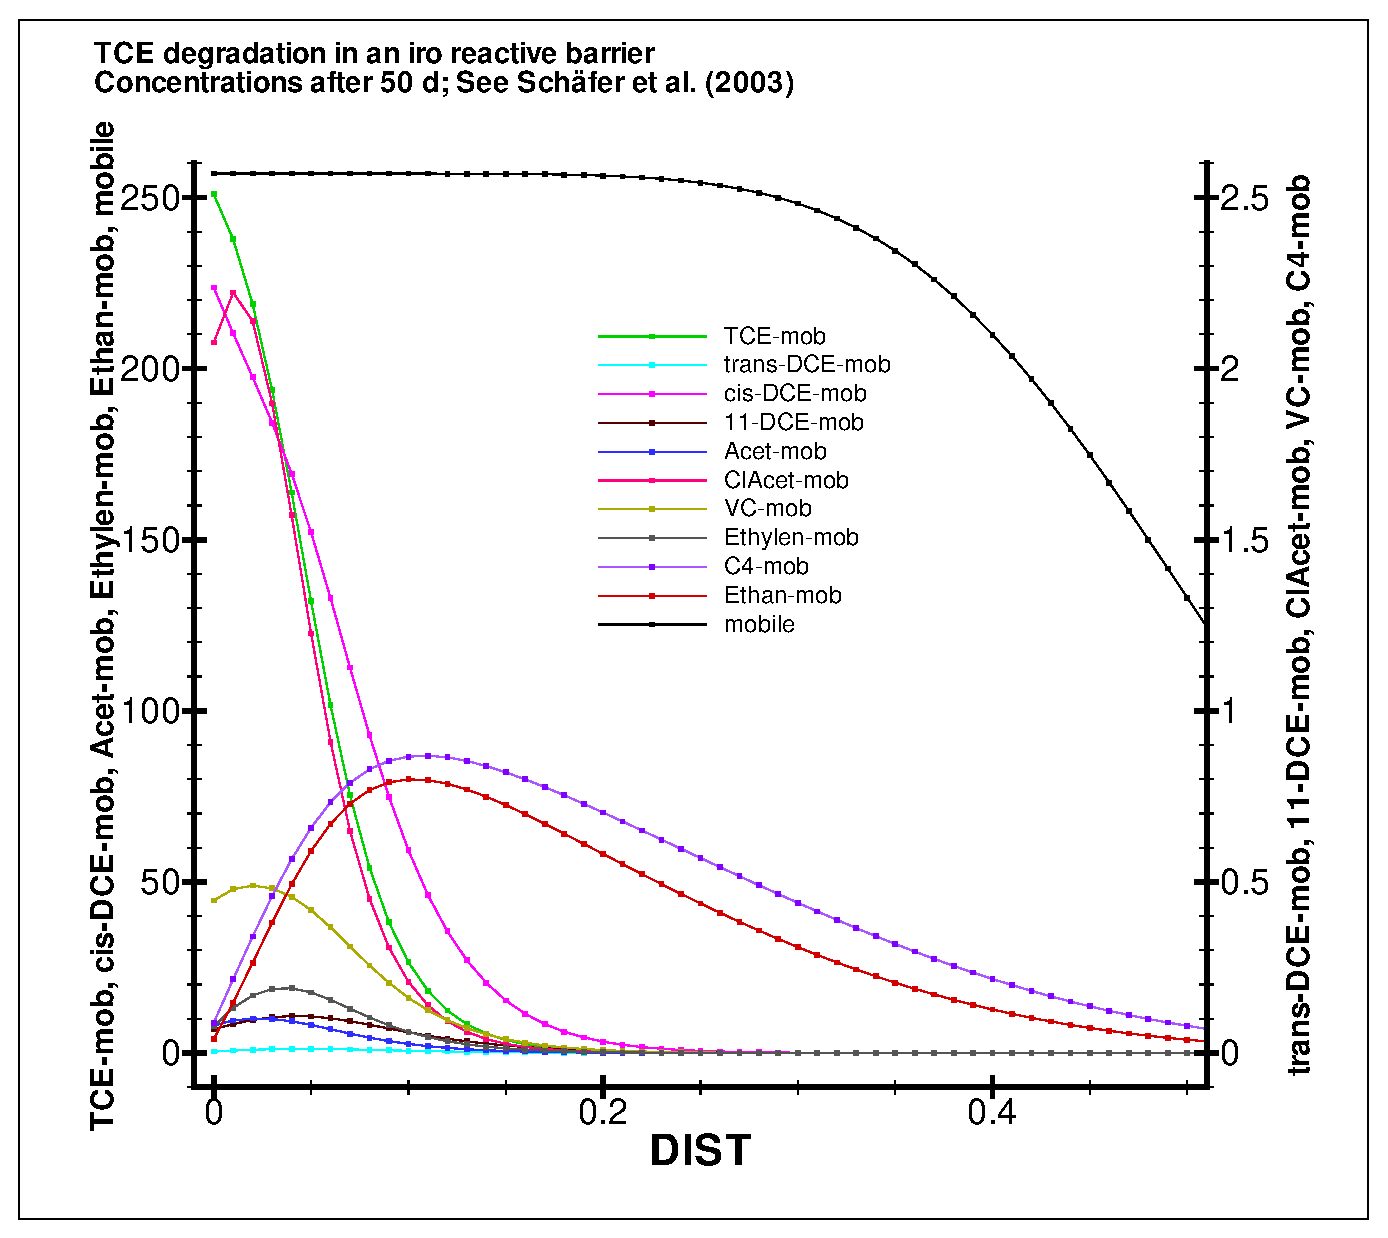
\includegraphics[width=0.9\textwidth]{PART_III/HC/1d_TCEonIon.eps}
\caption{Concentration profiles of TCE, trans-DCE, cis-DCE, 1,1-DCE, Acetylene, chloroacetylene, C4, VC, ethene and ethane as well as the concervative tracer mobile after 50 d simulation time.}
\label{profiles_TCEonIon}
\end{figure}
